%--------------------------------------------------------------
\section{Swagger na API}
%--------------------------------------------------------------
O Swagger, de acordo com sua documentação, é um \gls{framework} de código aberto que possui ferramentas que auxiliam na documentação dos serviços de uma \gls{REST API} com especificação \gls{openAPI}, o sistema deve apenas conter protocolos \acs{http} para aplica-lo, independente da linguagem que está sendo utilizada. O Swagger realiza a descrição de todos os recursos da \acs{api}, mostrando quais métodos \acs{http}, entidades, operações possíveis e parâmetros a serem enviados de cada \glspl{endpoint} da \gls{REST API}, por uma interface que a tecnologia disponibiliza, o Swagger UI. Portanto, este \gls{framework} facilita o entendimento do usuário em relação aos serviços de uma \acs{api}, proporcionando produtividade ao desenvolvedor.

Para a \acs{api} do projeto, está sendo utilizado a versão 3 do Swagger, pois esta versão é a mais atual e exige menos linhas de código para implementa-la, além de nos dar mais recursos, principalmente em relação à autenticidade do sistema, segundo sua documentação. O Swagger foi implementado em um arquivo dependências gerenciado pelo \gls{Maven}, após isso foi ajustada através de uma classe de configuração do \gls{SpringBoot} para geração do documento \gls{openAPI} do sistema. A \autoref{swagger API} mostra a interface do Swagger UI da \acs{api} que está sendo desenvolvida.

\begin{figure}[htb]
\centering
\caption{\label{swagger API} Swagger UI da API}
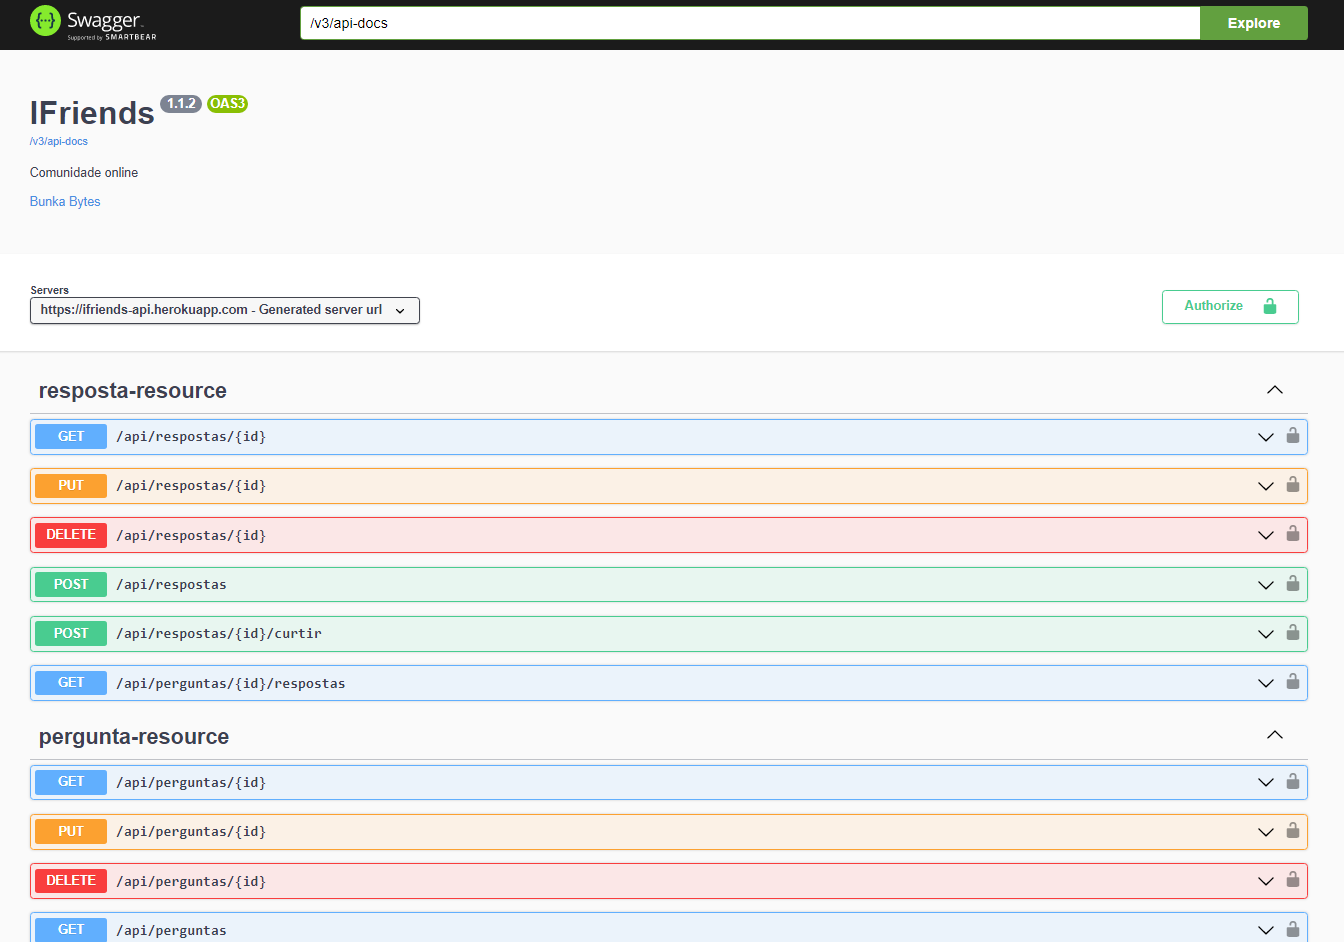
\includegraphics[width=1\textwidth]{anexos/Imagens_Swagger/API_swagger.png}
\fonte{os autores}
\end{figure}
\FloatBarrier

Como foi possível constatar na \autoref{swagger API}, no canto superior da interface indica informações gerais do projeto como o nome da \acs{api}, versão, descrição e nome da equipe. Já a parte inferior é mostrado o nome da classe de controle e a URI de cada requisição com seus métodos \acs{http}. O botão \textit{``Authorize''} é a principal função, pois este nos permite colocar o \acs{jwt} para verificar o usuário que está realizando a requisição. Após abrir um terminal, é apresentado os parâmetros, o corpo da requisição e a descrição da resposta com o código de estado, como é possível observar na \autoref{demostracao swagger API}.

\begin{figure}[htb]
\centering
\caption{\label{demostracao swagger API} Exemplo Swagger na API}
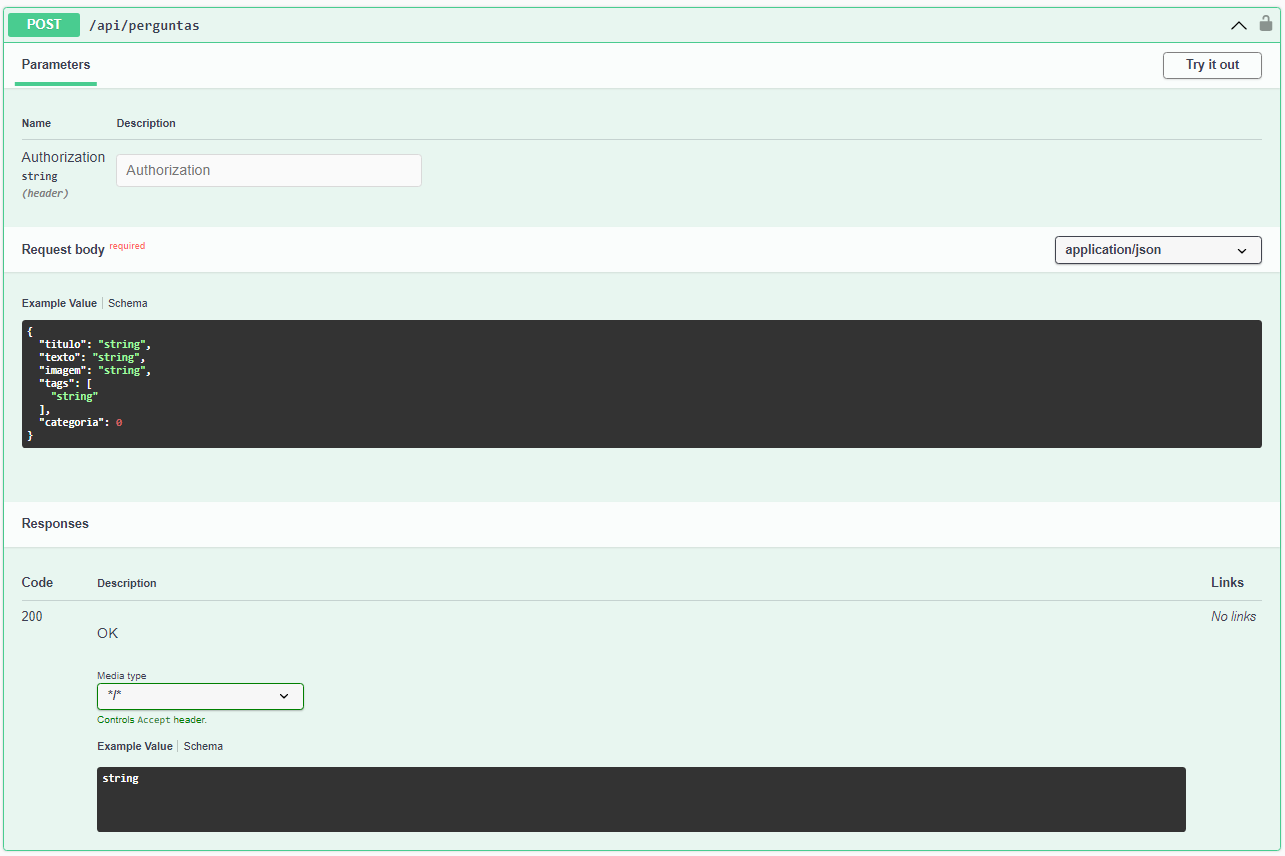
\includegraphics[width=1\textwidth]{anexos/Imagens_Swagger/API_swagger_demostracao.png}
\fonte{os autores}
\end{figure}
\FloatBarrier
